% Fakesection 序言之前

\RequirePackage[l2tabu, orthodox]{nag}
\RequirePackage{ifxetex}
\RequireXeTeX

\documentclass{article}

%颜色
\usepackage{xcolor}

%长度
\usepackage{printlen}
\uselengthunit{mm}

%图形
\usepackage{pifont}
\usepackage{ean13isbn}
\usepackage{qrcode}
\usepackage{pdfpages}
\usepackage{overpic}
\usepackage{graphicx}
\graphicspath{{fig/}{img/}{etc/}}
\usepackage{media9}
\usepackage{wallpaper}
\usepackage{wrapfig}

%表格
\usepackage{tabu}
\usepackage{longtable}
\usepackage{booktabs}
\usepackage{diagbox}
\usepackage{multicol}
\usepackage{multirow}
\usepackage{makecell}
\usepackage{fancybox}
\usepackage{colortbl}
\usepackage{tcolorbox}
\tcbuselibrary{skins}
\tcbuselibrary{breakable}
\tcbuselibrary{theorems}
\tcbuselibrary{listings}
\tcbuselibrary{xparse}
\tcbuselibrary{minted}% 用minted排版代码
\usepackage{fvextra}
\usepackage{csvsimple}
\usepackage{boxedminipage2e}

%公式
\usepackage{amsmath}
\usepackage{amsthm}
\usepackage{amsfonts}
\usepackage{amssymb}
\usepackage{amsbsy}
\usepackage{amsopn}
\usepackage{amstext}
\usepackage{mathrsfs}
\usepackage{bm}
\usepackage{textcomp}
\usepackage{latexsym}
\usepackage{exscale}
\usepackage{relsize}
%\usepackage{xymtex}
\usepackage{physics}
\usepackage{siunitx}
\usepackage{hologo}
\usepackage{cases}

%文字
\usepackage{csquotes}
\usepackage{microtype}
\usepackage[heading=true]{ctex}
\setCJKfamilyfont{zhsong}[AutoFakeBold = {2.17}]{SimSun}
\renewcommand*{\songti}{\CJKfamily{zhsong}}

%正文
\usepackage{fancyhdr}
\usepackage{geometry}
\usepackage{lastpage}
\usepackage{indentfirst}
\usepackage{setspace}
\renewcommand\arraystretch{1}

%非正文
\usepackage{makeidx}
\makeindex
\usepackage{epigraph}
\usepackage{varwidth}
\usepackage{exercise}
\usepackage{tasks}
\renewcommand{\ExerciseName}{实验题目}
\renewcommand{\AnswerName}{回答}
\renewcommand{\listexercisename}{实验题目}

%参考文献
\usepackage{morewrites}
\renewcommand{\thefootnote}{\fnsymbol{footnote}}
\usepackage[resetlabels]{multibib}

%标题
\usepackage{caption}
\usepackage{subcaption}
\DeclareCaptionLabelFormat{andtable}%
{#1#2~\&~\tablename\thetable}
\newcounter{sub}

%其它
\usepackage{atbegshi}
\usepackage{lipsum}

\csname
endofdump
\endcsname

%代码
\usepackage{minted}
\usepackage{boxie}
\makeatletter
\xdefinecolor{tcbcol@back}{rgb}{0,0,0}
\makeatother

%链接%与beamer 冲突
\usepackage[
colorlinks = true,
linkcolor = gray,
citecolor = gray,
backref=page
]{hyperref}

%枚举%与beamer 干涉
\usepackage{enumitem}
\setlist[enumerate, 2]{
	fullwidth,
	label = \arabic*.,
	font = \textup,
	itemindent=2em
}

%标题%与beamer 冲突
\usepackage{titlesec}
%\titleformat{\chapter}{\centering\Huge\bfseries}{实验\chinese{chapter}~}{0pt}{}
\titleformat{\section}{\centering\LARGE\bfseries}{\S\ifthenelse{\value{section}=0}{}{\thesection}~}{0pt}{}
%\titleformat{\subsection}{\Large}{\chinese{subsection}、~}{0pt}{}
%\titleformat{\subsubsection}{\large}{\arabic{subsubsection}.~}{0pt}{}

\begin{document}

% Fakesection 扉页

\begin{titlepage}
	\centering

	\includegraphics[width=.8\linewidth]{NJUST.ai}

	\vspace{20mm}

	\begin{spacing}{1.5}

		\centering

		\textbf{\songti\zihao{1}电子工程与光电技术学院}

		\vspace{5mm}

		\textbf{\songti\zihao{1}实验报告}

		\vspace{20mm}

		\zihao{-2}

		\begin{tabu}to.8\linewidth{@{}X[4,r]@{}X[c]@{}X[12,l]@{}}
			\makebox[4\ccwd][s]{课程名称}      & :&\underline{\makebox[12\ccwd][c]{\kaishu 电子信息工程综合实验}}\\
			\makebox[4\ccwd][s]{实验名称}      & :&\underline{\makebox[12\ccwd][c]{\kaishu 仿真线性调频脉冲雷达系统}}\\
			\makebox[4\ccwd][s]{班级}      & :&\underline{\makebox[12\ccwd][c]{\kaishu 9161042101}}\\
			\makebox[4\ccwd][s]{小组成员}  & :&\underline{\makebox[12\ccwd][c]{\kaishu 邹顺宇 9161630R0127}}\\
			\makebox[4\ccwd][s]{}  & &\underline{\makebox[12\ccwd][c]{\kaishu 吴振宇 916101630117}}\\
			\makebox[4\ccwd][s]{}  & &\underline{\makebox[12\ccwd][c]{\kaishu 周世峰 916104330154}}\\
			\makebox[4\ccwd][s]{指导老师}      & :&\underline{\makebox[12\ccwd][c]{\kaishu 李洪涛}}
		\end{tabu}
		\vspace{0mm}%缩进

	\end{spacing}

	\vspace{0mm}%缩进

	\zihao{4}

	\today

\end{titlepage}

%页眉页脚%与book冲突
\pagestyle{fancy}
\renewcommand{\headrulewidth}{0pt}
\lhead{\small{\leftmark}}
\chead{\small{\rightmark}}
\rhead{\small{第\thepage 页~共~\pageref{LastPage}~页}}
\lfoot{}
\cfoot{}
\rfoot{}

% Fakesection 目录

\pagenumbering{roman}

\tableofcontents
\listoffigures
\listoftables
\listofexercises

\setcounter{section}{-1}

\pagenumbering{arabic}

\newpage

\section{实验要求}%
\label{sec:实验要求}

\begin{Exercise}
	雷达技术要求:

	\begin{tabu}to.8\linewidth{@{}X[6,r]@{}X[c]@{}X[10,l]@{}}
		\makebox[6\ccwd][l]{目标探测距离} & :&\makebox[10\ccwd][l]{$ \geqslant \SI{3}{km} $}\\
		\makebox[6\ccwd][l]{近距离盲区}   & :&\makebox[10\ccwd][l]{$ \leqslant \SI{200}{m} $}\\
		\makebox[6\ccwd][l]{测速范围}     & :&\makebox[10\ccwd][l]{$ \SI{4}{m/s}\sim \SI{100}{m/s} $}\\
		\makebox[6\ccwd][l]{速度分辨力}   & :&\makebox[10\ccwd][l]{\SI{4}{m/s}}\\
		\makebox[6\ccwd][l]{距离分辨力}   & :&\makebox[10\ccwd][l]{\SI{10}{m}}\\
		\makebox[6\ccwd][l]{RCS}          & :&\makebox[10\ccwd][l]{$ \SI{0.01}{m^2} $}\\
	\end{tabu}

	\kaishu 根据要求设计雷达的$ T_r $、$ \tau $、脉冲积累点数$ N $、发射功率$ P_t $及带宽等参数。

	\vspace{0mm}

\end{Exercise}

\section{实验材料}%
\label{sec:实验材料}

\subsection{硬件材料}%
\label{sub:硬件材料}

本次实验基于江苏万邦微电子有限公司设计的雷达信号分析与处理综合试验箱进行。\cite{instrument}

\begin{figure}[H]
	\centering
	\begin{subfigure}[H]{.45\linewidth}
		\centering
		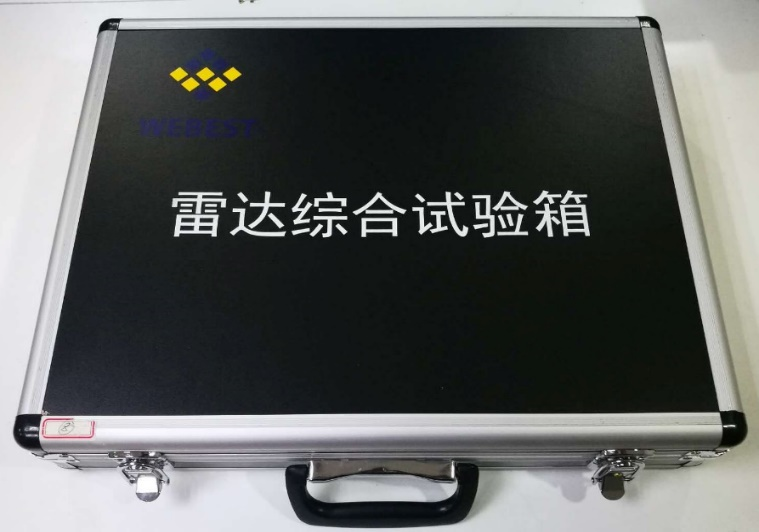
\includegraphics[width=\linewidth]{hardwareOuter.png}
		\caption{试验箱外观}
		\label{fig:试验箱外观}
	\end{subfigure}
	\quad
	\begin{subfigure}[H]{.45\linewidth}
		\centering
		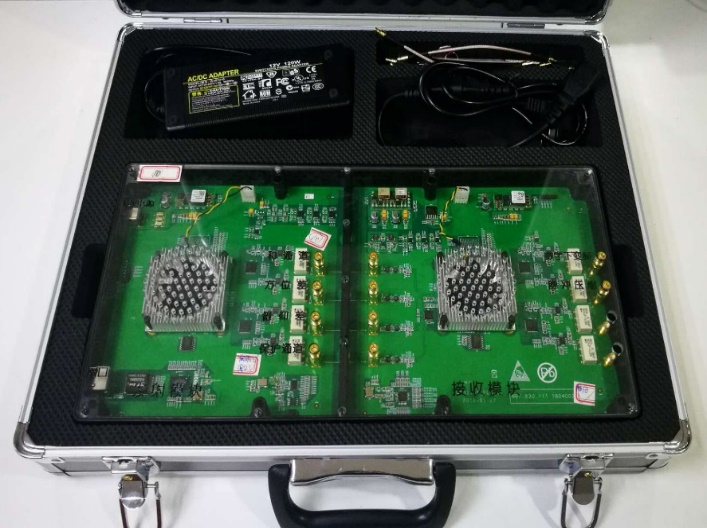
\includegraphics[width=\linewidth]{hardwareInner.png}
		\caption{试验箱内部}
		\label{fig:试验箱内部}
	\end{subfigure}
	\caption{试验箱}
	\label{fig:试验箱}
\end{figure}

\begin{description}
	\item[用途:] 《雷达原理》必修实验所需实验装置;
	\item[功能:] 可实现各种常用波形(LFM、二相编码等)的信号处理各个流程的仿真,包括生成中频回波、数字下变频、脉冲压缩、MTI、MTD、CFAR、单脉冲比幅测角,最终输出目标点迹。
\end{description}

\subsection{软件材料}%
\label{sub:软件材料}

软件可显示各信号处理节点的波形或处理结果,硬件可输出各信号处理节点的波形,并可通过网口回传处理结果给上位机软件。

\begin{description}
	\item[控制:]
		\begin{enumerate}
			\item 配置波形参数、目标参数、算法参数等;
			\item 通过网口发送命令报文,实现对系统的控制;
		\end{enumerate}
	\item[信号产生及处理:] 完成信号产生及处理流程的仿真;
	\item[显示:]
		\begin{enumerate}
			\item 显示信号产生及处理各流程的波形或处理结果;
			\item 显示试验箱回传的目标信息。
		\end{enumerate}
\end{description}

\section{实验原理}%
\label{sec:实验原理}

\subsection{雷达工作原理}%
\label{sub:雷达工作原理}

雷达主要是通过发射机产生符合要求的雷达波形,然后经馈线和收发开关由发射天线辐射出去,遇到目标之后,一部分电磁波发生反射,经接收天线和收发开关由接收机接收回波信号,通过对雷达信号做适当的处理即可获知目标的距离、俯仰角、速度、形态特征等相关信息。\cite{radar}

在本实验中,我们仅考虑目标的距离与速度等参量。假设目标与雷达的相对距离为$ R $,发射信号为$ S(t) $,为了探测到该目标,雷达发射机将发射信号以光速$ c $向四周传播,经过时间$ t=\dfrac{R}{c} $后发射信号到达目标。此时发射信号的表达式为$ s(t-\dfrac{R}{c}) $。发射信号接触到目标后,一部分被目标吸收,另一部分被目标散射,其中被目标散射的信号可以表示为$ \sigma s(t-\dfrac{R}{c}) $,其中$ \sigma $为目标的雷达截面积,该信号我们在本实验中将其称为回波信号。回波信号再经过$ t=\dfrac{R}{c} $的时间,被雷达的接收机所接收,接收的信号表达式为$ s_r(t)=\sigma s(t-\dfrac{2R}{c}) $。

对于接收到的回波信号$ s_r(t)=\sigma s(t-\dfrac{2R}{c}) $,需要从中提取出表征目标特性的距离等参数,常用的方法是将信号$ s_r(t) $通过一个匹配滤波器。$ s_r(t) $的匹配滤波器为$ h_r(t)=s^*(-t) $,所以通过匹配滤波器后的信号为$ s_o(t)=h_r(t)*s_r(t) $。

对通过匹配滤波器后的信号进行频域分析,进行傅里叶变换$ S_o(\jmath\omega)=|S(\jmath\omega)|^2H(\jmath\omega) $。

通过选取合适的$ s(t) $,使其幅值特性为常数,从而可以得到$ S_0(\jmath\omega)=kH(\jmath\omega) $,再进行傅里叶逆变换$ s_o(t)=kh(t)=k\sum\limits_{i=1}^M\sigma_i\delta(t-\tau_i) $。

通过分析$ s_o(t) $我们可以得到我们想要的目标特征信息。

\subsection{线性调频脉冲信号}%
\label{sub:线性调频脉冲信号}

脉冲压缩雷达能同时提高雷达的作用距离和距离分辨率。这种体制采用宽脉冲发射以提高发射的平均功率,保证足够大的作用距离;而接受时采用相应的脉冲压缩算法获得窄脉冲,以提高距离分辨率,较好的解决雷达作用距离与距离分辨率之间的矛盾。

脉冲压缩雷达最常见的调制信号是线性调频信号,接收时采用匹配滤波器压缩脉冲。LFM信号的数学表达式为$ s(t)=\mathrm{Rect}(\dfrac{t}{T})\mathrm{e}^{2\jmath\pi(f_ct+\dfrac{k}{2}t^2) } $。

其中$ f_c $为载波频率,$ k=\dfrac{B}{T} $为调频斜率,$ \mathrm{Rect}(t) $为矩形信号。

为了方便对LFM信号进行处理,$ s(t) $信号可以重写为$ s(t)=S(t) \mathrm{e}^{2\jmath\pi f_ct} $。

其中,$ S(t)= \mathrm{Rect}(\dfrac{t}{T}) \mathrm{e}^{\jmath\pi kt^2} $是信号$ s(t) $的复包络,由傅里叶变换的性质可知,$ s(t) $和$ S(t) $虽然中心频率不同,但是具有相同的幅频特性,所以通过处理后的线性调频脉冲信号仿真时,只需考虑$ S(t) $。

\section{系统设计}%
\label{sec:系统设计}

\begin{table}[H]
	\centering
	\caption{系统设计}
	\csvautobooktabular{tab/parameter.csv}
	\label{tab:系统设计}
\end{table}

\subsection{距离分辨度}%
\label{sub:距离分辨度}

LFM脉冲雷达的距离分辨力为$ \Delta R=\dfrac{c}{2B} $;其中$ c $为光速,$ B $为发射信号的带宽。

实验要求距离分辨力为\SI{10}{m},计算得带宽至少为\SI{15}{MHz}。系统最后所取得带宽为\SI{20}{MHz}。

\subsection{速度分辨度}%
\label{sub:速度分辨度}

LFM脉冲雷达的速度分辨力则和相干积累总时宽以及信号时宽有关,当信号时宽越大,速度的分辨力就越高。有以下公式:

\begin{align}
	f_d=\dfrac{1}{NT}
\end{align}

其中$ T $为信号时宽,$ N $为相干积累的脉冲个数。由此可以得到理论上的最小可检测速度为$ v_{min}=f_d\dfrac{c}{2f_c} $,系统默认载频$ f_c=\SI{16}{\GHz} $。

实验要求速度分辨率为\SI{4}{\m/\s}。经过计算,当取信号的时宽T=\SI{100}{\us},相干积累脉冲个数为32时,可达到精度要求,为\SI{3.9}{m/s}。最大可测速度为\SI{124.8}{\m/\s},满足实验的测速范围要求。

\subsection{探测距离}%
\label{sub:探测距离}

通过查阅相关资料可知,LFM脉冲雷达的最大测距为$ R_{max}= \dfrac{cT_r}{2} $;其中$ c $为光速,$ T_r $为发射信号的时宽。

实验要求测距范围大于\SI{3}{\km},系统选取$ T_r=\SI{75}{\us} $,可测得\SI{11.25}{\km},满足要求。

\subsection{探测盲区}%
\label{sub:探测盲区}

通过查阅相关资料可知,LFM脉冲雷达的测距盲区为$ R_{min}= \dfrac{c\tau}{2} $;其中$ c $为光速,$ \tau $为发射信号脉冲时宽。

实验要求盲区小于\SI{200}{\m},则计算得脉冲时宽最大为\SI{1.33}{\us},同时考虑到发射机的发射功率和脉冲时宽成反比,脉冲时宽越大,发射功率越低,所以脉冲时宽选择\SI{0.6}{\us}。

\section{系统仿真}%
\label{sec:系统仿真}

\subsection{单目标仿真}%
\label{sub:单目标仿真}

\subsubsection{单目标中频信号}%
\label{ssub:单目标中频信号}

\begin{figure}[H]
	\centering
	\begin{subfigure}[H]{.45\linewidth}
		\centering
		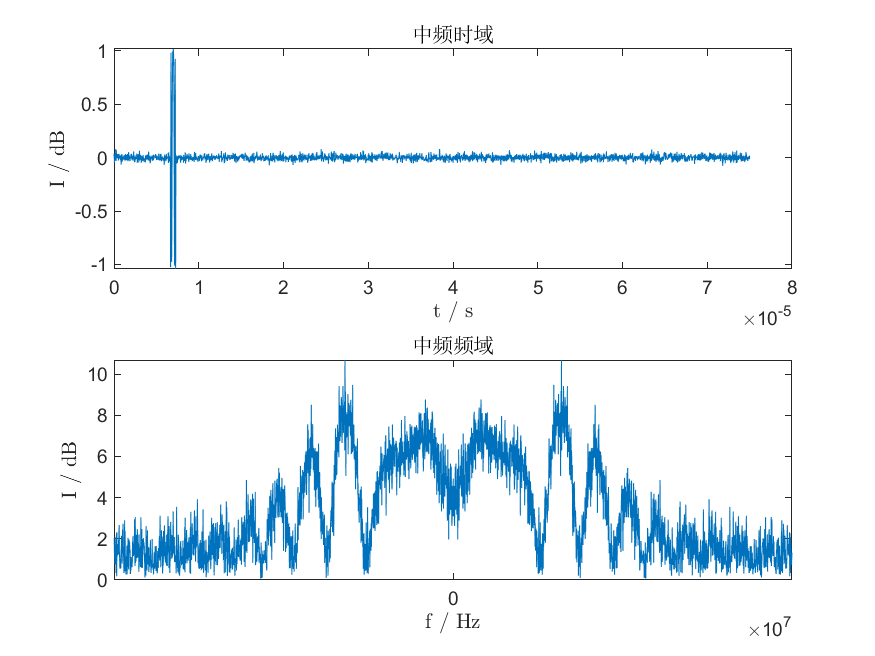
\includegraphics[width=\linewidth]{one-MF-matlab.png}
		\caption{单目标中频信号matlab仿真}
		\label{fig:单目标中频信号matlab仿真}
	\end{subfigure}
	\quad
	\begin{subfigure}[H]{.45\linewidth}
		\centering
		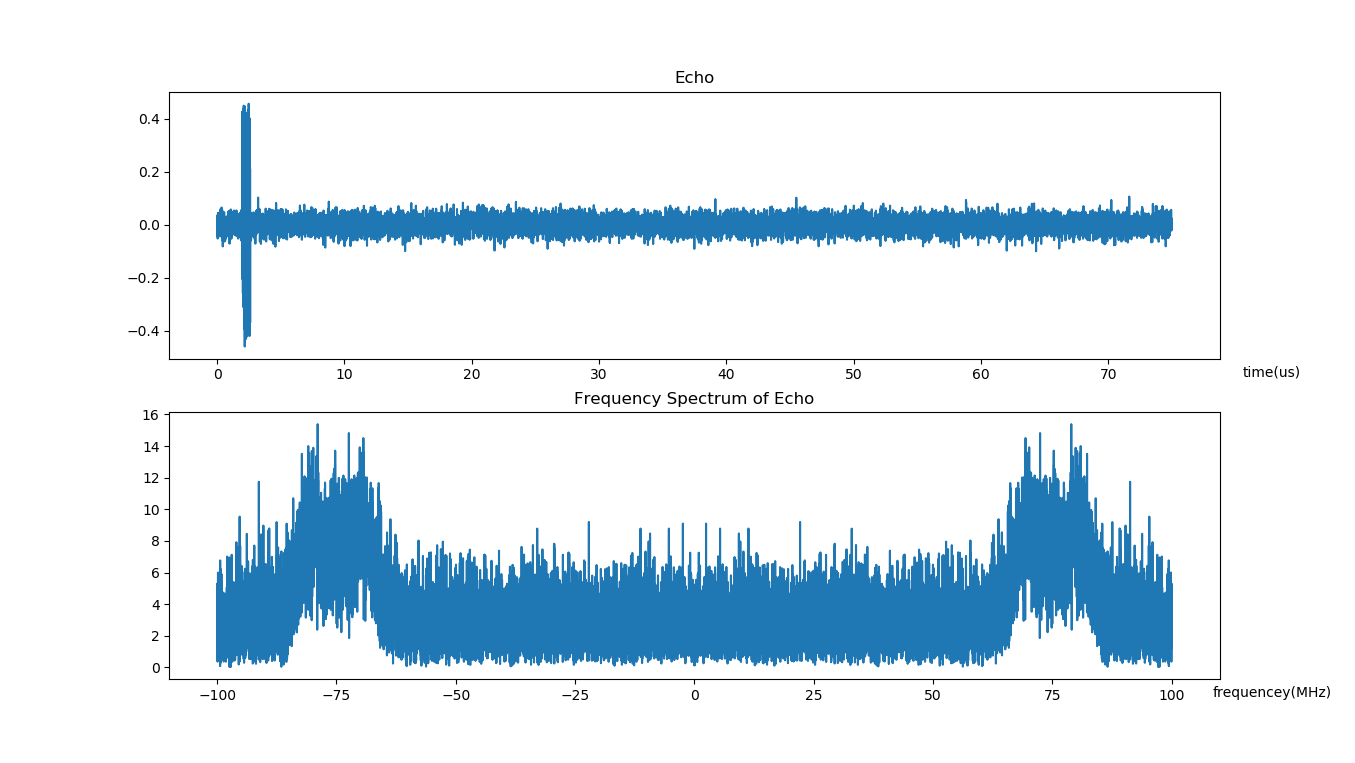
\includegraphics[width=\linewidth]{one-MF-software.png}
		\caption{单目标中频信号软件仿真}
		\label{fig:单目标中频信号软件仿真}
	\end{subfigure}
	\quad
	\begin{subfigure}[H]{.45\linewidth}
		\centering
		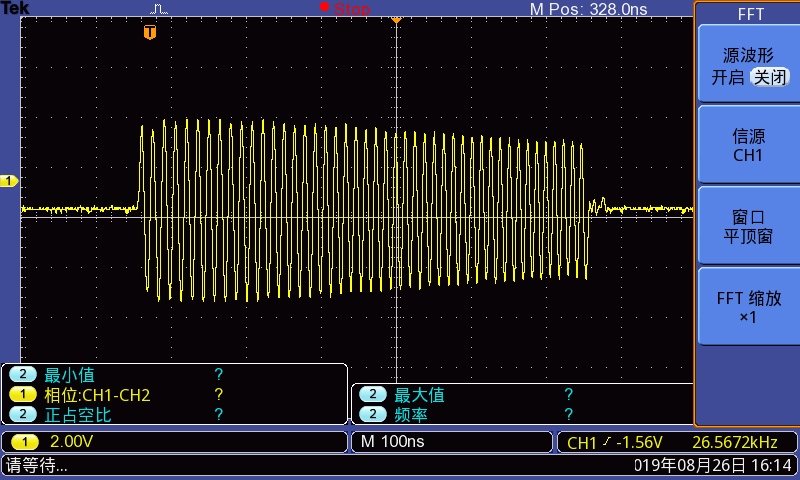
\includegraphics[width=\linewidth]{one-MF-hardware.png}
		\caption{单目标中频信号硬件仿真}
		\label{fig:单目标中频信号硬件仿真}
	\end{subfigure}
	\caption{单目标中频信号}
	\label{fig:单目标中频信号}
\end{figure}

\subsubsection{单目标脉冲压缩信号}%
\label{ssub:单目标脉冲压缩信号}

\begin{figure}[H]
	\centering
	\begin{subfigure}[H]{.45\linewidth}
		\centering
		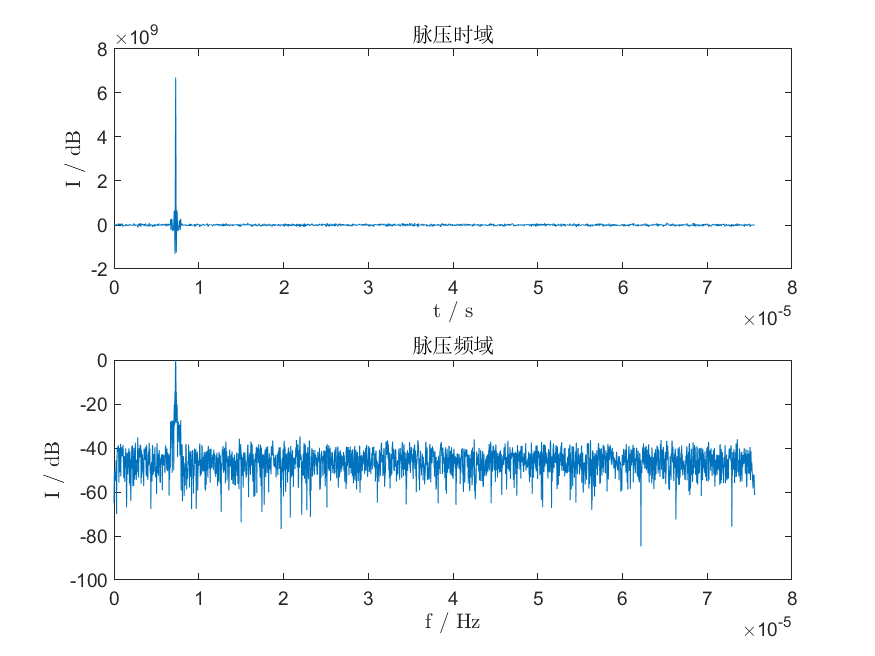
\includegraphics[width=\linewidth]{one-pulse-matlab.png}
		\caption{单目标脉冲压缩信号matlab仿真}
		\label{fig:单目标脉冲压缩信号matlab仿真}
	\end{subfigure}
	\quad
	\begin{subfigure}[H]{.45\linewidth}
		\centering
		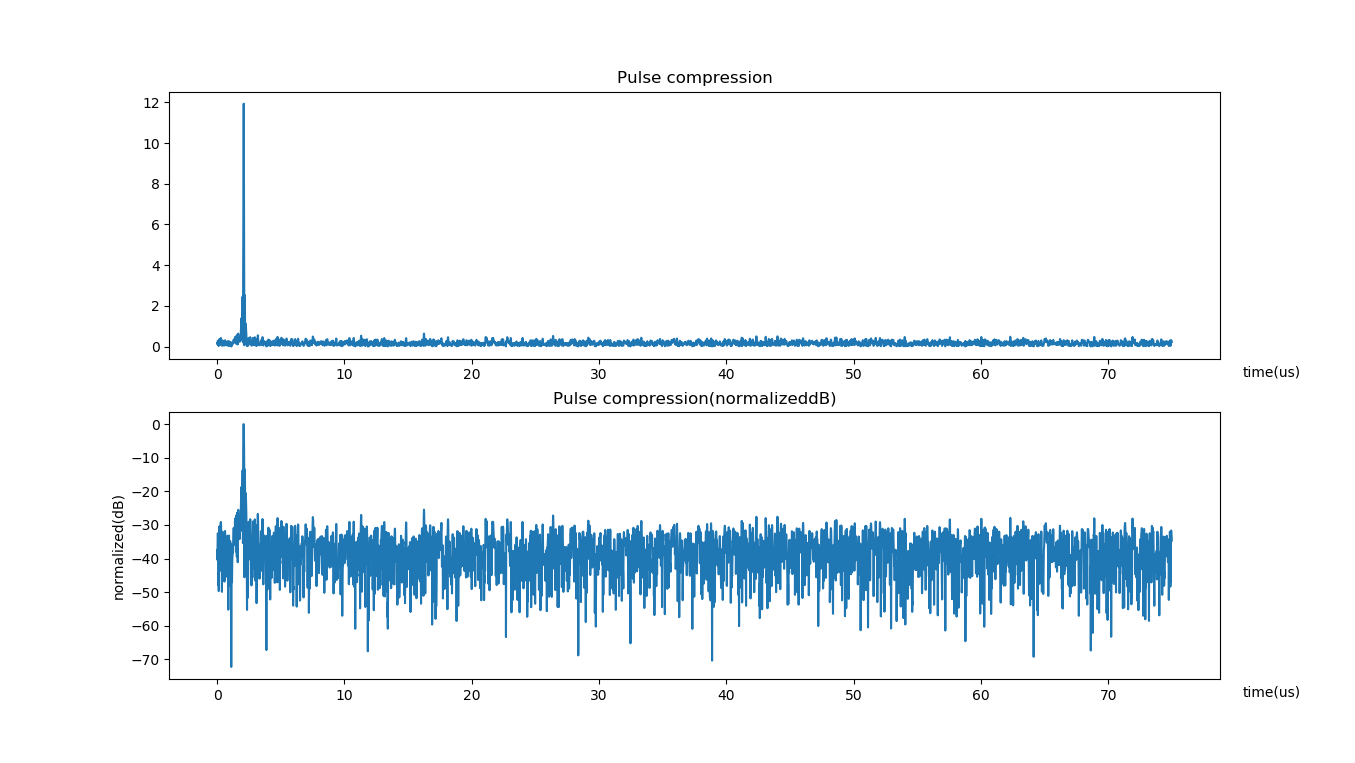
\includegraphics[width=\linewidth]{one-pulse-software.png}
		\caption{单目标脉冲压缩信号软件仿真}
		\label{fig:单目标脉冲压缩信号软件仿真}
	\end{subfigure}
	\quad
	\begin{subfigure}[H]{.45\linewidth}
		\centering
		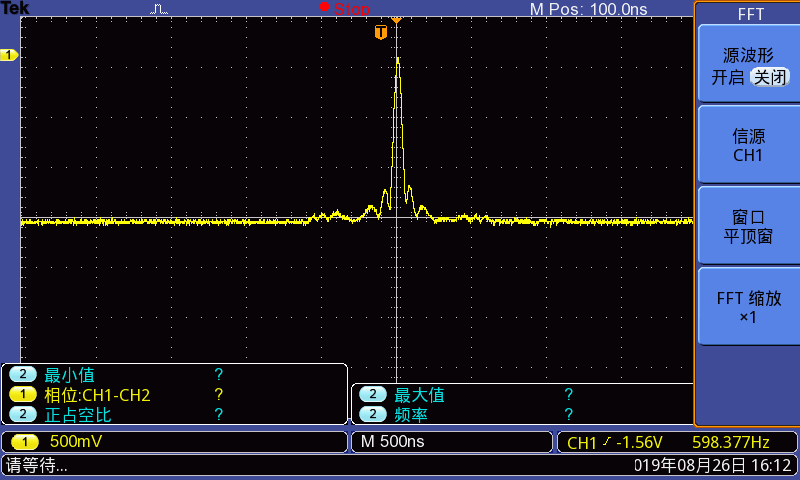
\includegraphics[width=\linewidth]{one-pulse-hardware.png}
		\caption{单目标脉冲压缩信号硬件仿真}
		\label{fig:单目标脉冲压缩信号硬件仿真}
	\end{subfigure}
	\caption{单目标脉冲压缩信号}
	\label{fig:单目标脉冲压缩信号}
\end{figure}

\subsubsection{单目标基带信号}%
\label{ssub:单目标基带信号}

\begin{figure}[H]
	\centering
	\begin{subfigure}[H]{.45\linewidth}
		\centering
		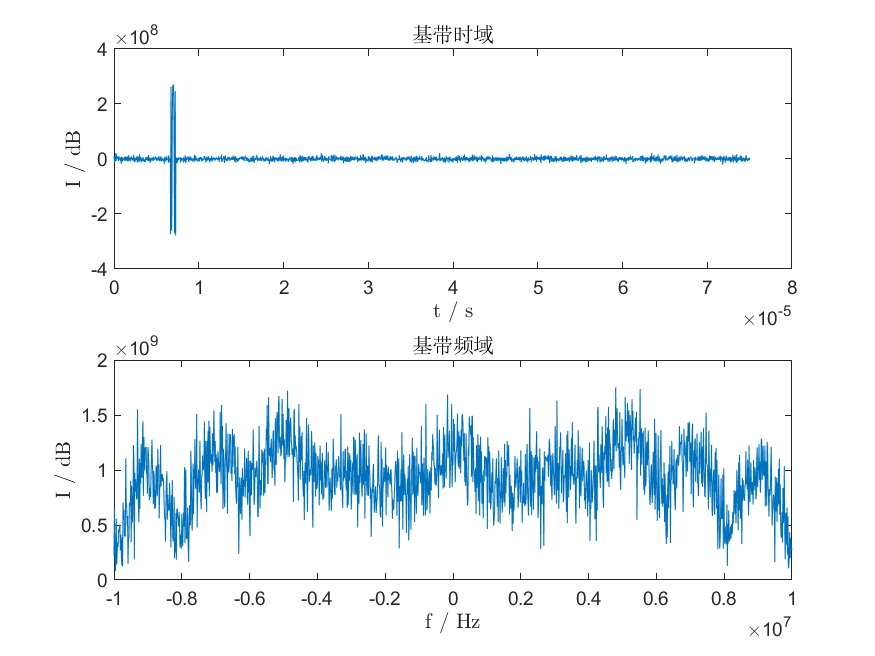
\includegraphics[width=\linewidth]{one-baseband-matlab.png}
		\caption{单目标基带信号matlab仿真}
		\label{fig:单目标基带信号matlab仿真}
	\end{subfigure}
	\quad
	\begin{subfigure}[H]{.45\linewidth}
		\centering
		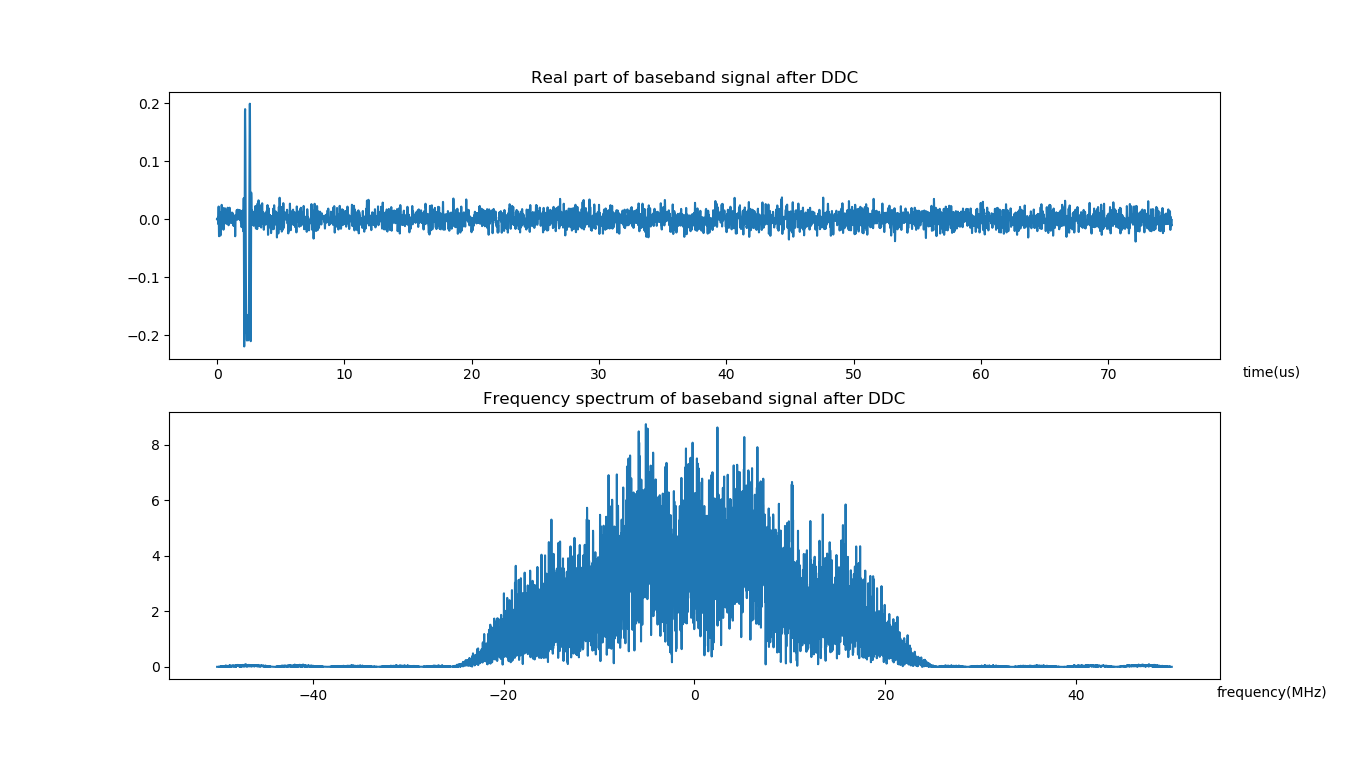
\includegraphics[width=\linewidth]{one-baseband-software.png}
		\caption{单目标基带信号软件仿真}
		\label{fig:单目标基带信号软件仿真}
	\end{subfigure}
	\quad
	\begin{subfigure}[H]{.45\linewidth}
		\centering
		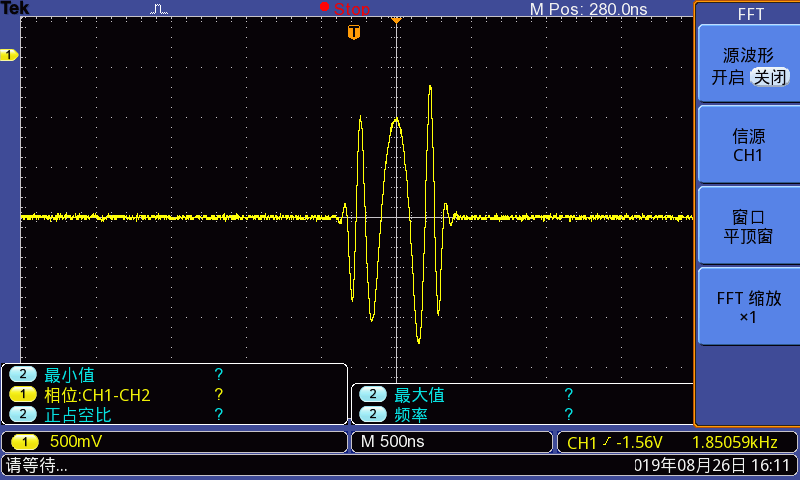
\includegraphics[width=\linewidth]{one-baseband-hardware.png}
		\caption{单目标基带信号硬件仿真}
		\label{fig:单目标基带信号硬件仿真}
	\end{subfigure}
	\caption{单目标基带信号}
	\label{fig:单目标基带信号}
\end{figure}

\subsection{单目标动态目标检测}%
\label{sub:单目标动态目标检测}

\begin{figure}[H]
	\centering
	\begin{subfigure}[H]{.6\linewidth}
		\centering
		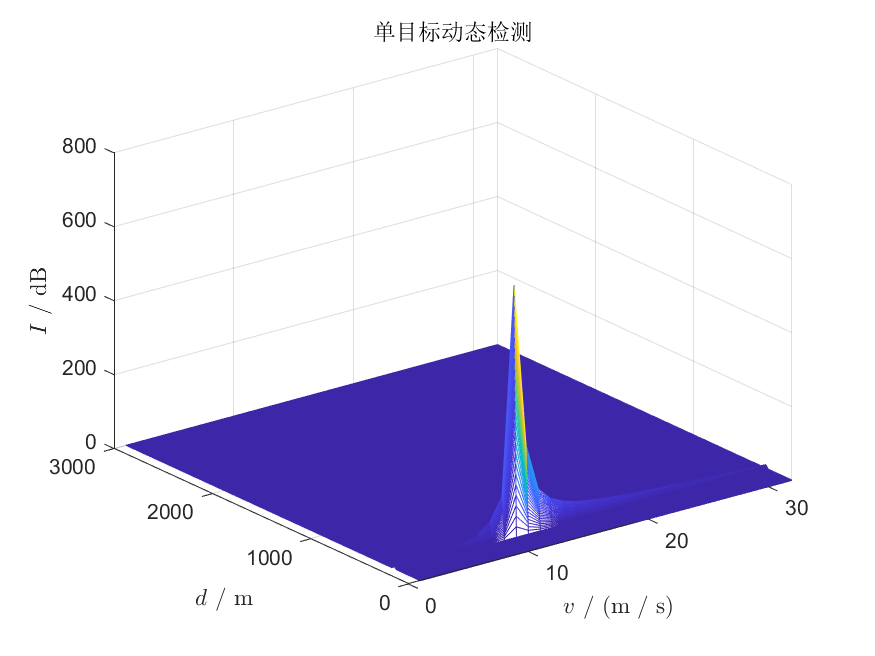
\includegraphics[width=\linewidth]{one-MTD-matlab.png}
		\caption{单目标动态目标检测matlab仿真}
		\label{fig:单目标动态目标检测matlab仿真}
	\end{subfigure}
	\quad
	\begin{subfigure}[H]{.6\linewidth}
		\centering
		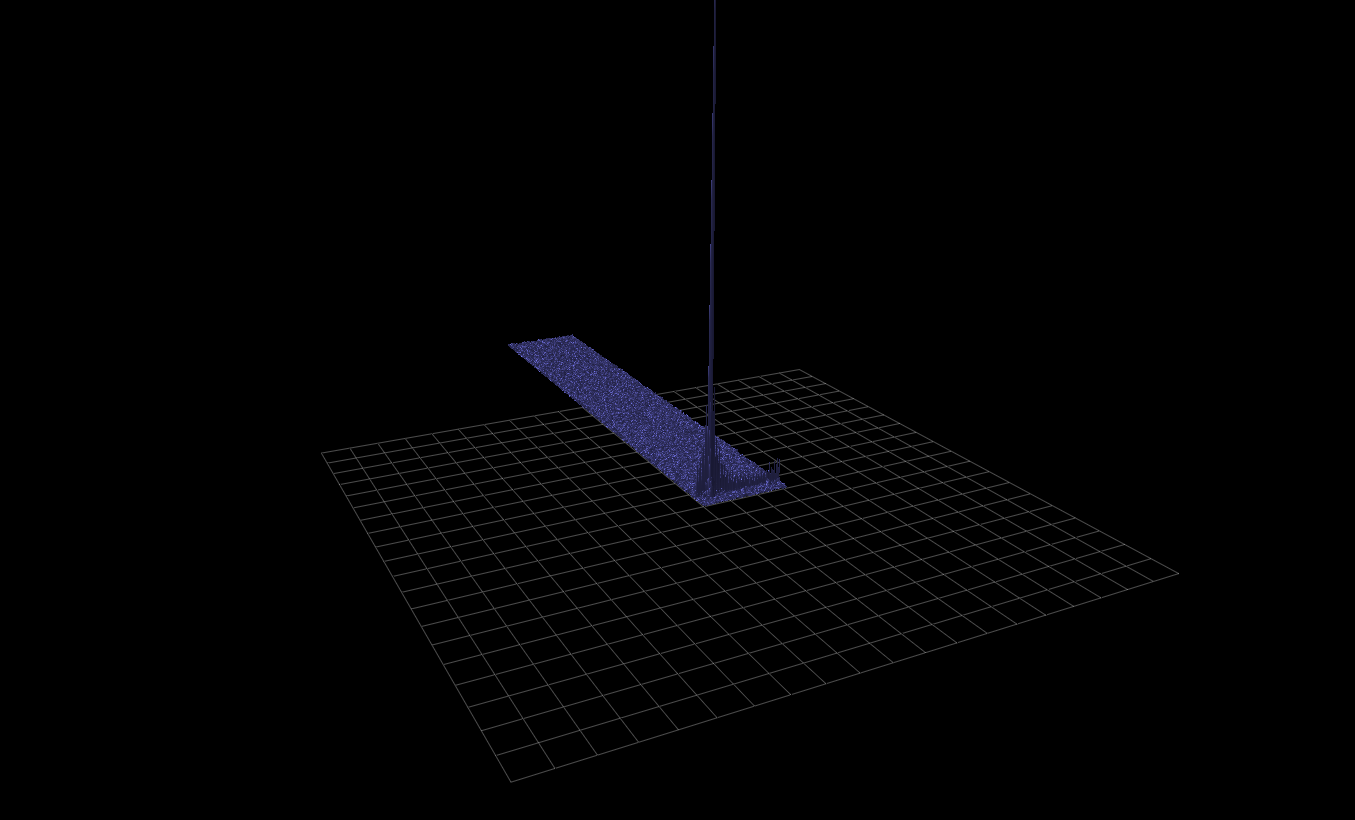
\includegraphics[width=\linewidth]{one-MTD-software.png}
		\caption{单目标动态目标检测软件仿真}
		\label{fig:单目标动态目标检测软件仿真}
	\end{subfigure}
	\caption{单目标动态目标检测}
	\label{fig:单目标动态目标检测}
\end{figure}

\subsection{多目标仿真}%
\label{sub:多目标仿真}

\subsubsection{多目标中频信号}%
\label{ssub:多目标中频信号}

\begin{figure}[H]
	\centering
	\begin{subfigure}[H]{.45\linewidth}
		\centering
		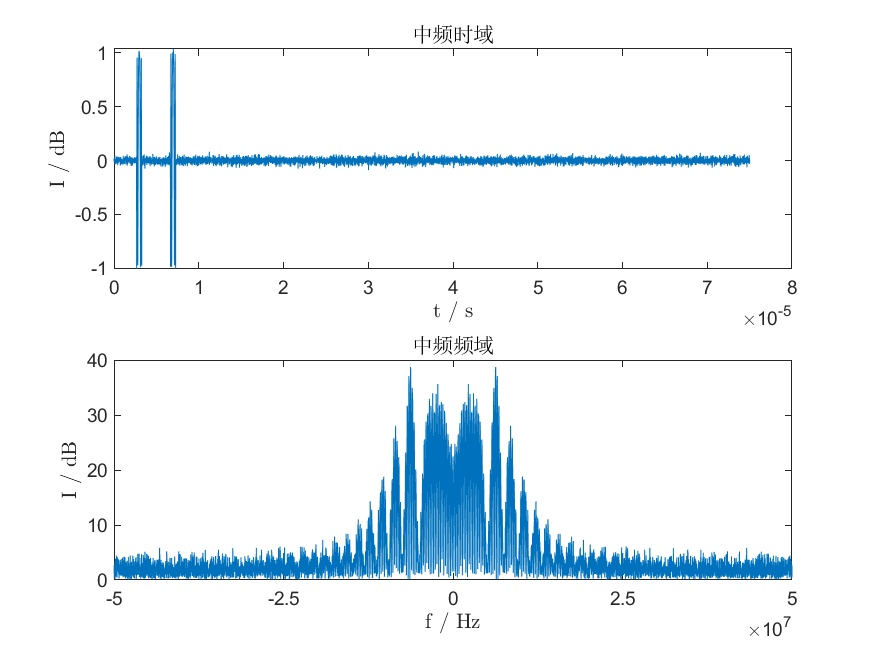
\includegraphics[width=\linewidth]{two-MF-matlab.png}
		\caption{多目标中频信号matlab仿真}
		\label{fig:多目标中频信号matlab仿真}
	\end{subfigure}
	\quad
	\begin{subfigure}[H]{.45\linewidth}
		\centering
		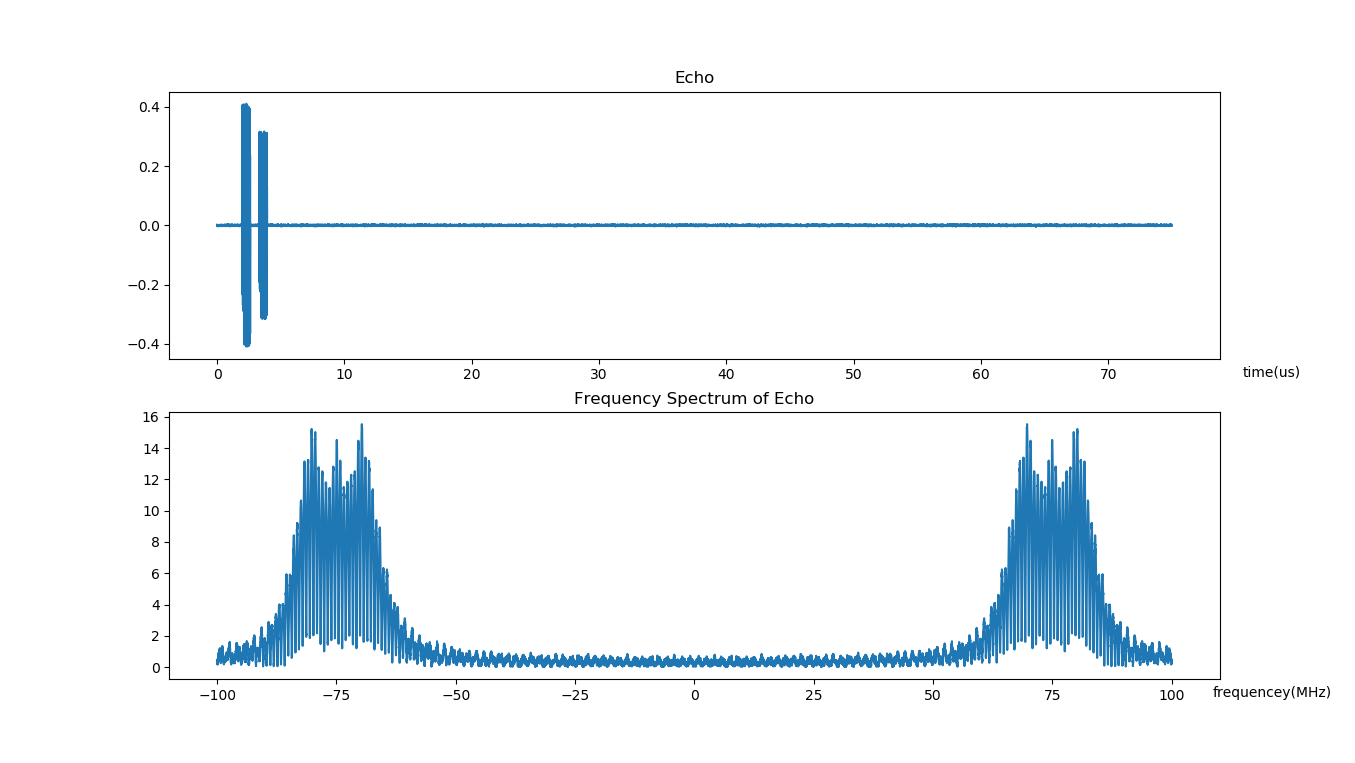
\includegraphics[width=\linewidth]{two-MF-software.png}
		\caption{多目标中频信号软件仿真}
		\label{fig:多目标中频信号软件仿真}
	\end{subfigure}
	\quad
	\begin{subfigure}[H]{.45\linewidth}
		\centering
		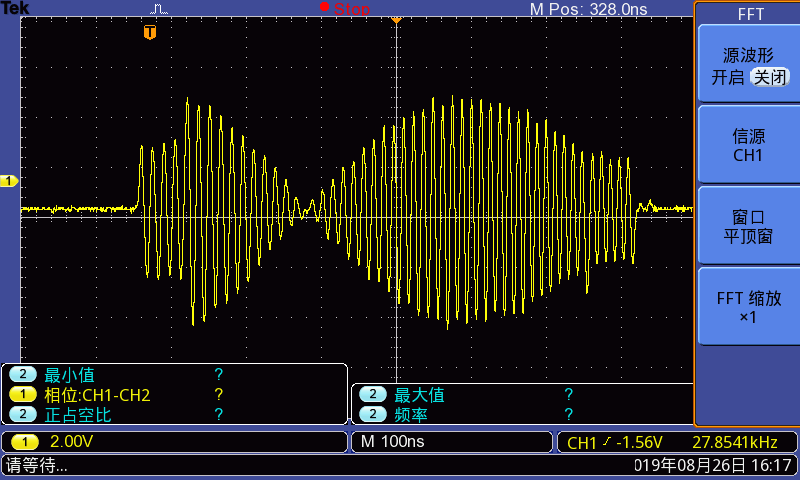
\includegraphics[width=\linewidth]{two-MF-hardware.png}
		\caption{多目标中频信号硬件仿真}
		\label{fig:多目标中频信号硬件仿真}
	\end{subfigure}
	\caption{多目标中频信号}
	\label{fig:多目标中频信号}
\end{figure}

\subsubsection{多目标脉冲压缩信号}%
\label{ssub:多目标脉冲压缩信号}

\begin{figure}[H]
	\centering
	\begin{subfigure}[H]{.45\linewidth}
		\centering
		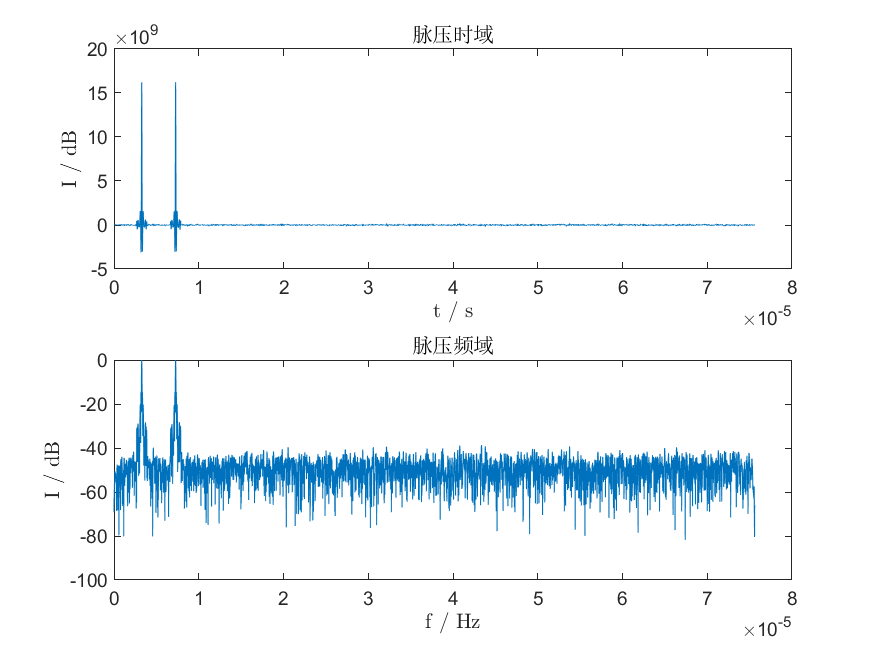
\includegraphics[width=\linewidth]{two-pulse-matlab.png}
		\caption{多目标脉冲压缩信号matlab仿真}
		\label{fig:多目标脉冲压缩信号matlab仿真}
	\end{subfigure}
	\quad
	\begin{subfigure}[H]{.45\linewidth}
		\centering
		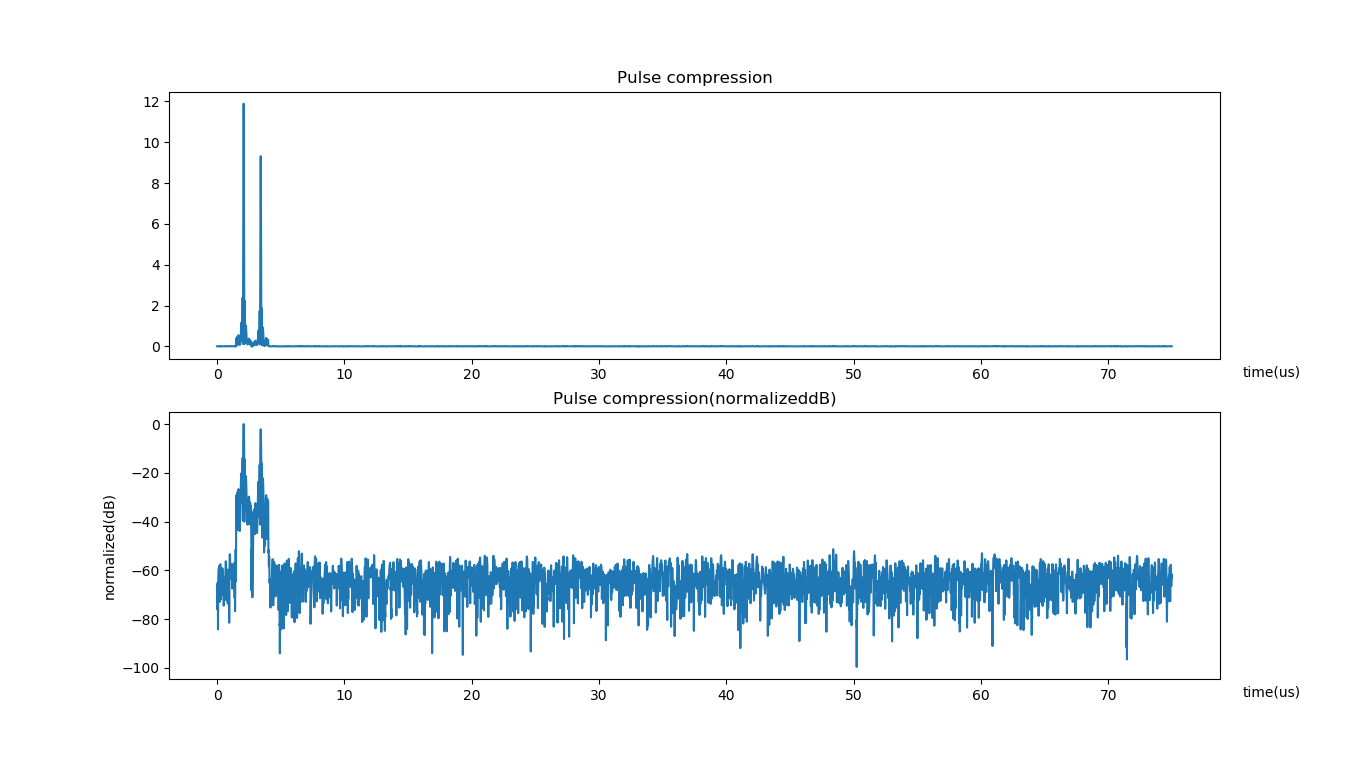
\includegraphics[width=\linewidth]{two-pulse-software.png}
		\caption{多目标脉冲压缩信号软件仿真}
		\label{fig:多目标脉冲压缩信号软件仿真}
	\end{subfigure}
	\quad
	\begin{subfigure}[H]{.45\linewidth}
		\centering
		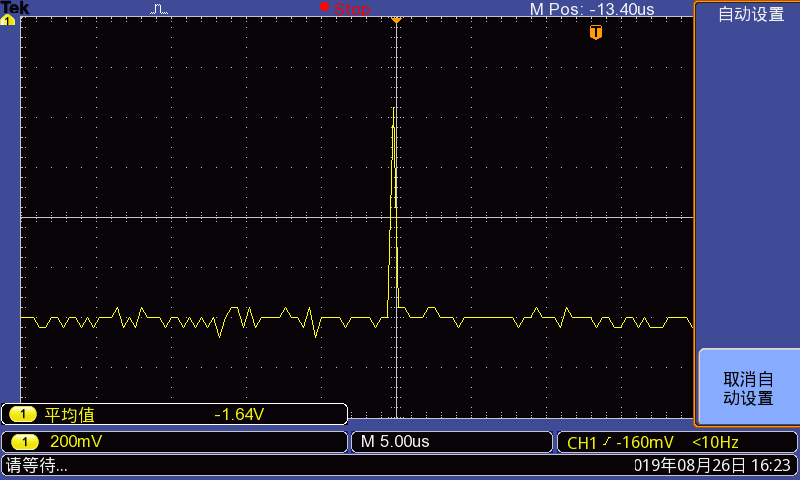
\includegraphics[width=\linewidth]{two-pulse-hardware.png}
		\caption{多目标脉冲压缩信号硬件仿真}
		\label{fig:多目标脉冲压缩信号硬件仿真}
	\end{subfigure}
	\caption{多目标脉冲压缩信号}
	\label{fig:多目标脉冲压缩信号}
\end{figure}

\subsubsection{多目标基带信号}%
\label{ssub:多目标基带信号}

\begin{figure}[H]
	\centering
	\begin{subfigure}[H]{.45\linewidth}
		\centering
		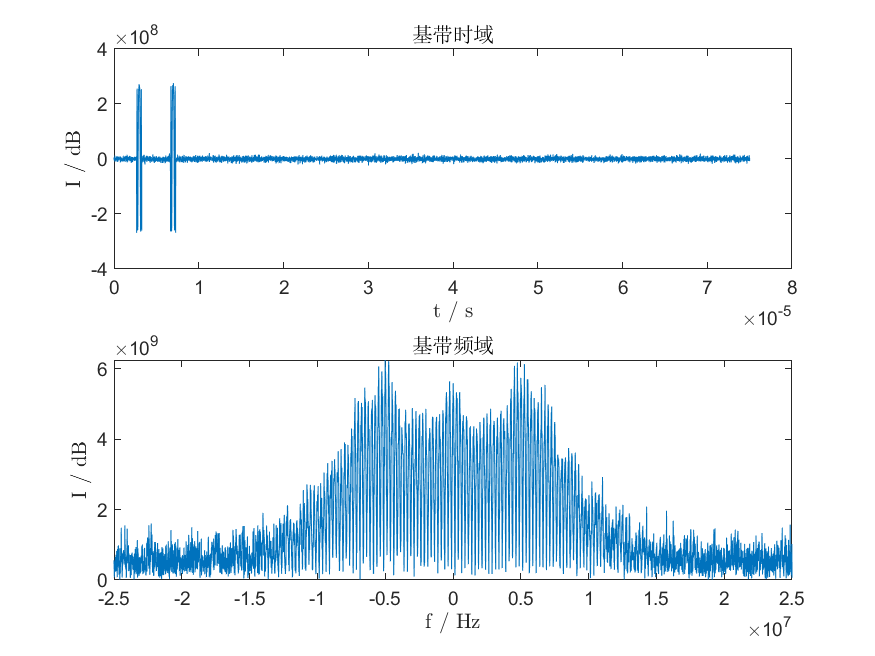
\includegraphics[width=\linewidth]{two-baseband-matlab.png}
		\caption{多目标基带信号matlab仿真}
		\label{fig:多目标基带信号matlab仿真}
	\end{subfigure}
	\quad
	\begin{subfigure}[H]{.45\linewidth}
		\centering
		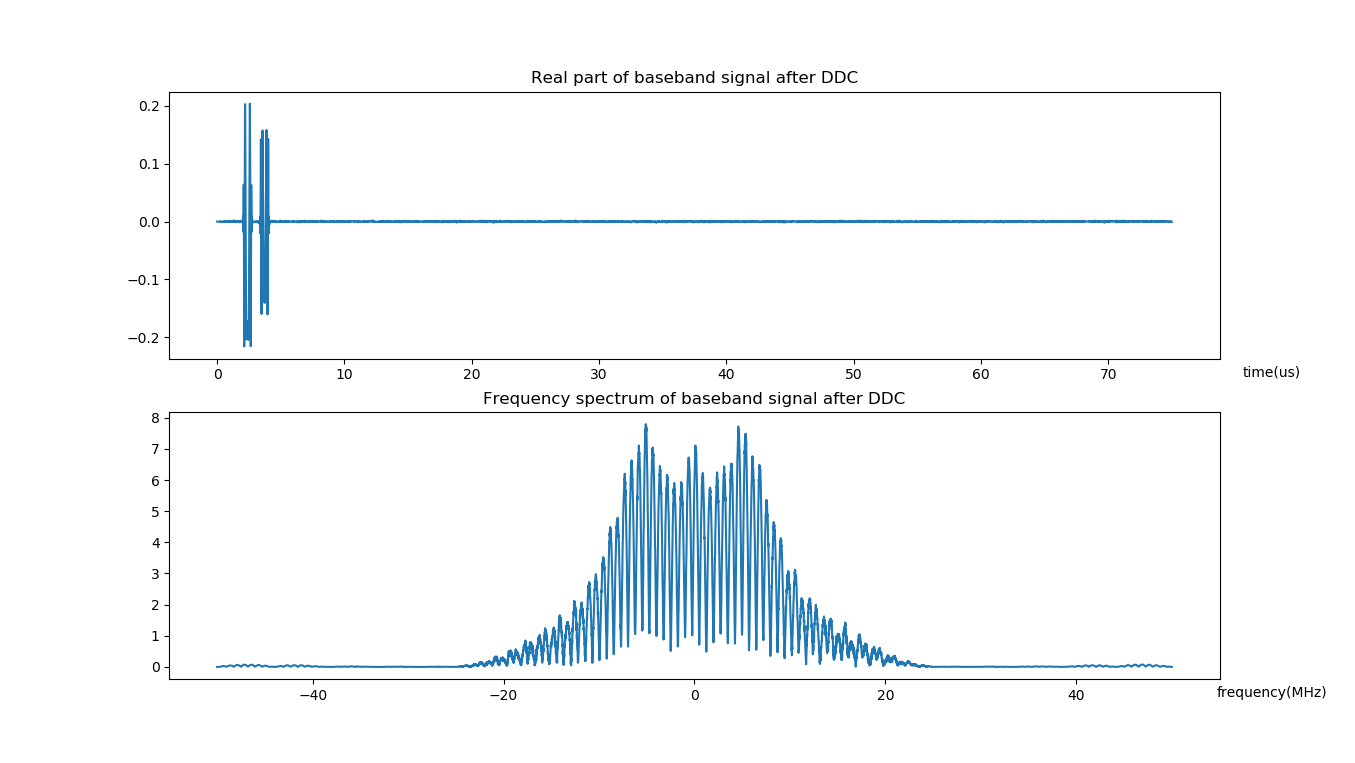
\includegraphics[width=\linewidth]{two-baseband-software.png}
		\caption{多目标基带信号软件仿真}
		\label{fig:多目标基带信号软件仿真}
	\end{subfigure}
	\quad
	\begin{subfigure}[H]{.45\linewidth}
		\centering
		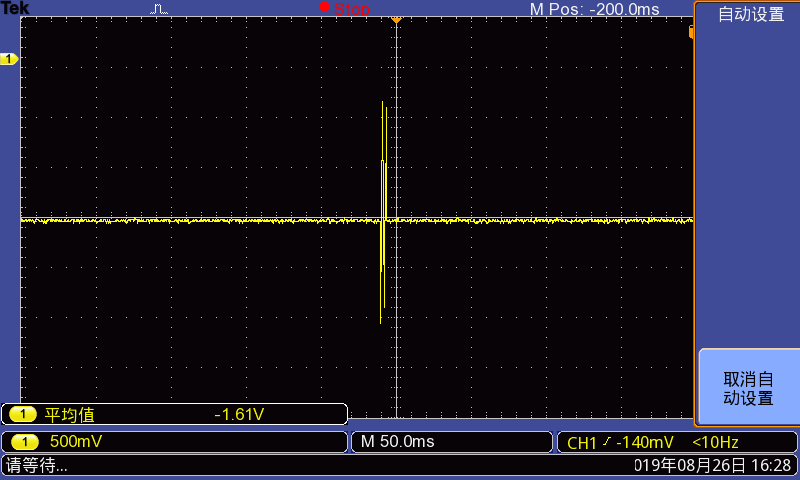
\includegraphics[width=\linewidth]{two-baseband-hardware.png}
		\caption{多目标基带信号硬件仿真}
		\label{fig:多目标基带信号硬件仿真}
	\end{subfigure}
	\caption{多目标基带信号}
	\label{fig:多目标基带信号}
\end{figure}

\subsection{多目标动态目标检测}%
\label{sub:多目标动态目标检测}

\begin{figure}[H]
	\centering
	\begin{subfigure}[H]{.6\linewidth}
		\centering
		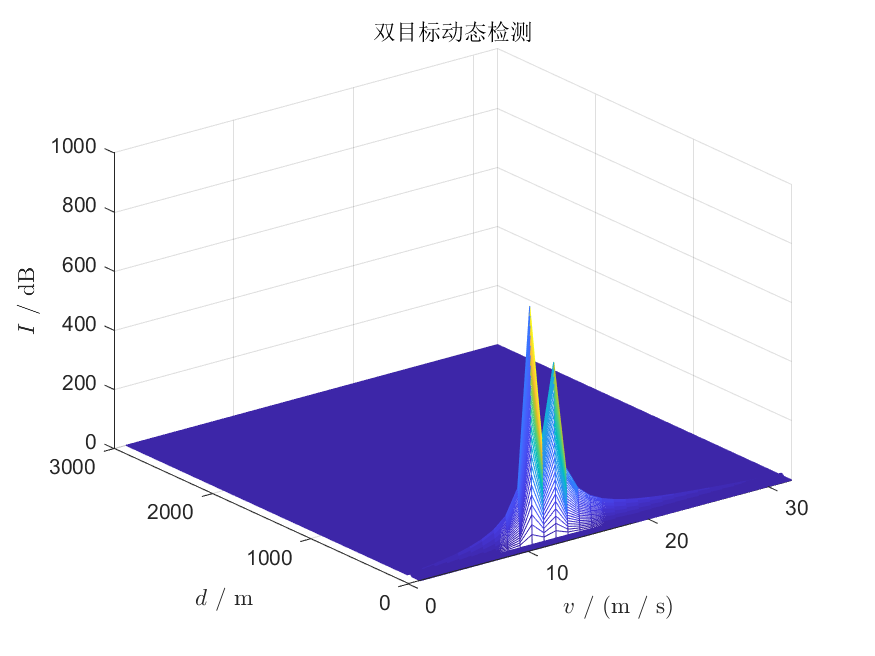
\includegraphics[width=\linewidth]{two-MTD-matlab.png}
		\caption{多目标动态目标检测matlab仿真}
		\label{fig:多目标动态目标检测matlab仿真}
	\end{subfigure}
	\quad
	\begin{subfigure}[H]{.6\linewidth}
		\centering
		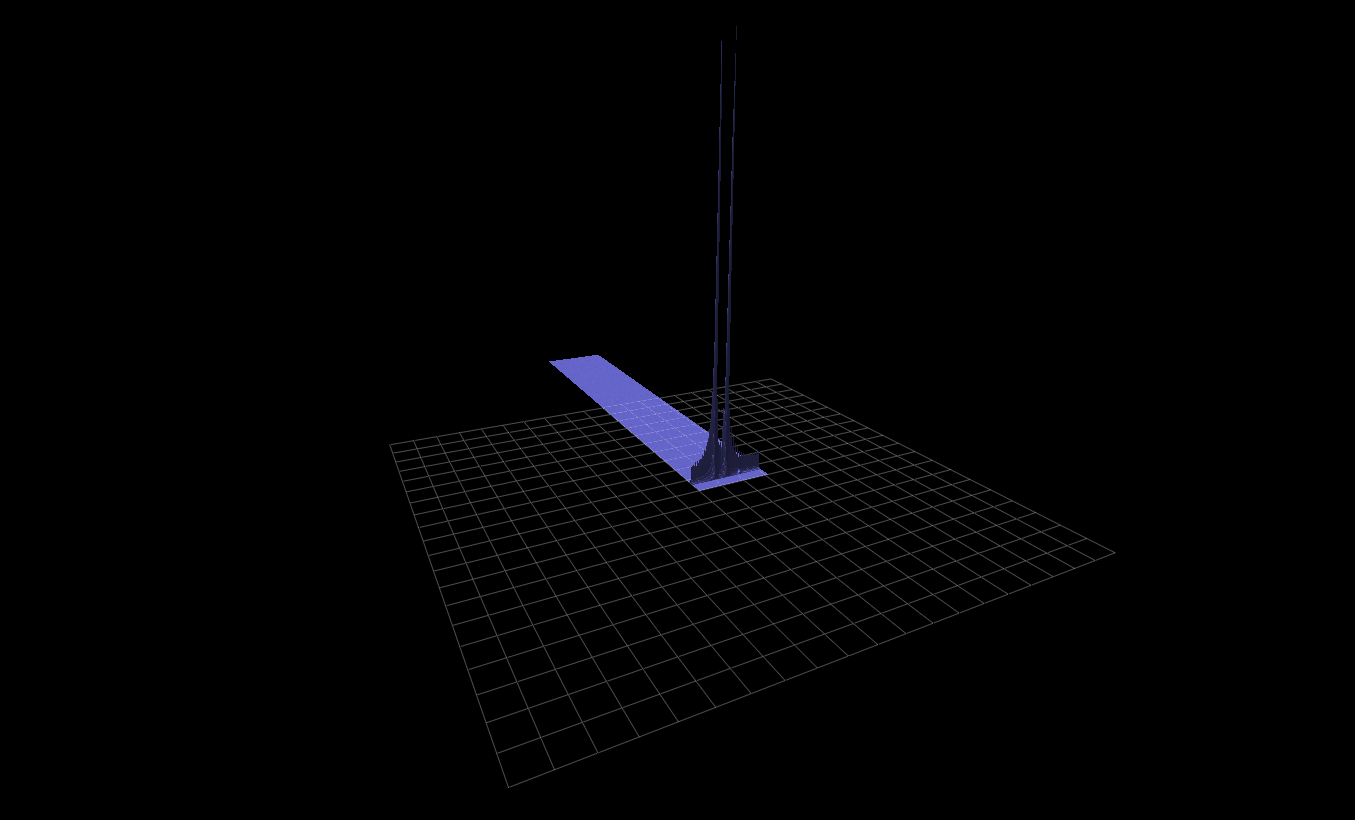
\includegraphics[width=\linewidth]{two-MTD-software.png}
		\caption{多目标动态目标检测软件仿真}
		\label{fig:多目标动态目标检测软件仿真}
	\end{subfigure}
	\caption{多目标动态目标检测}
	\label{fig:多目标动态目标检测}
\end{figure}

\subsection{速度分辨}%
\label{sub:速度分辨}

\begin{figure}[H]
	\centering
	\begin{subfigure}[H]{.45\linewidth}
		\centering
		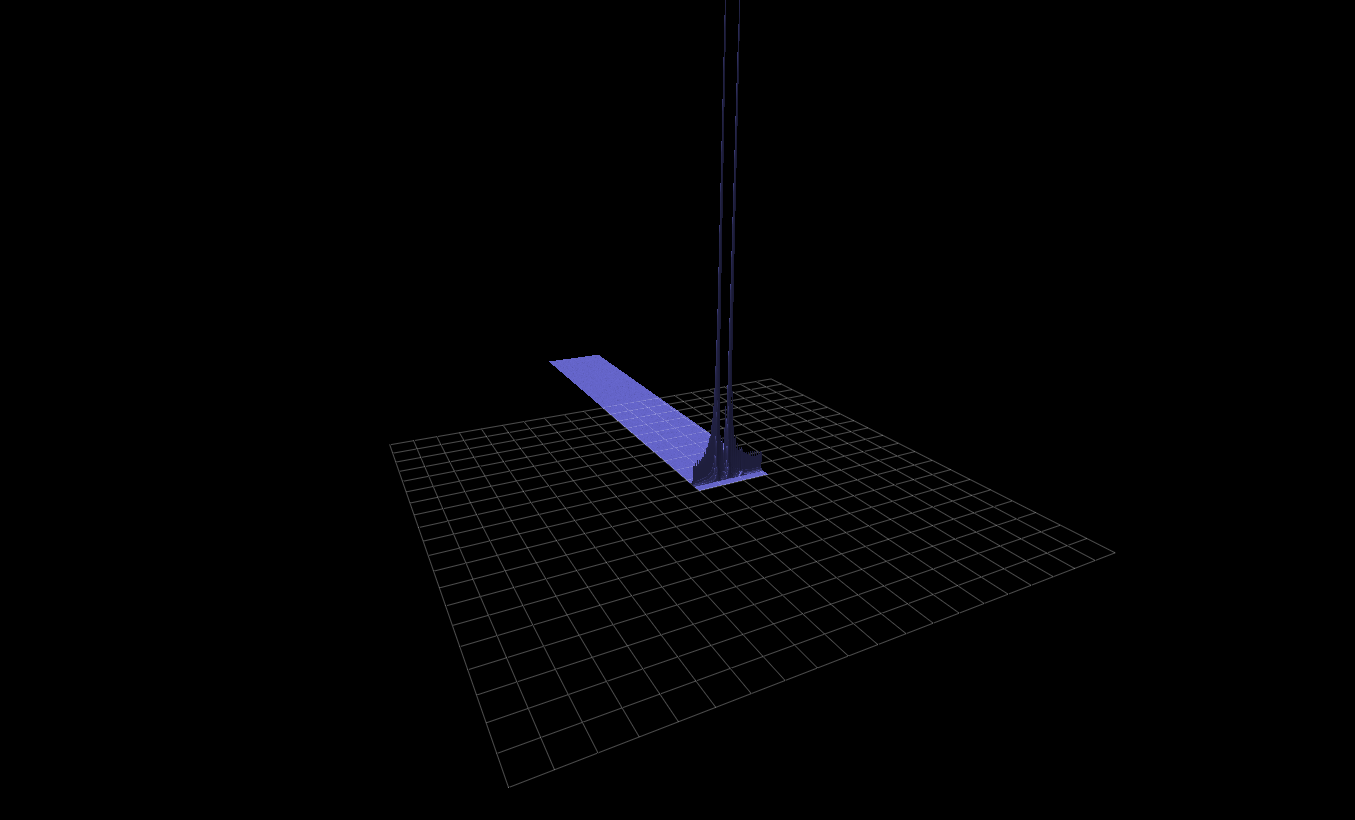
\includegraphics[width=\linewidth]{vector20-MTD-software.png}
		\caption{两目标速度差为20m/s}
		\label{fig:两目标速度差为20m/s}
	\end{subfigure}
	\quad
	\begin{subfigure}[H]{.45\linewidth}
		\centering
		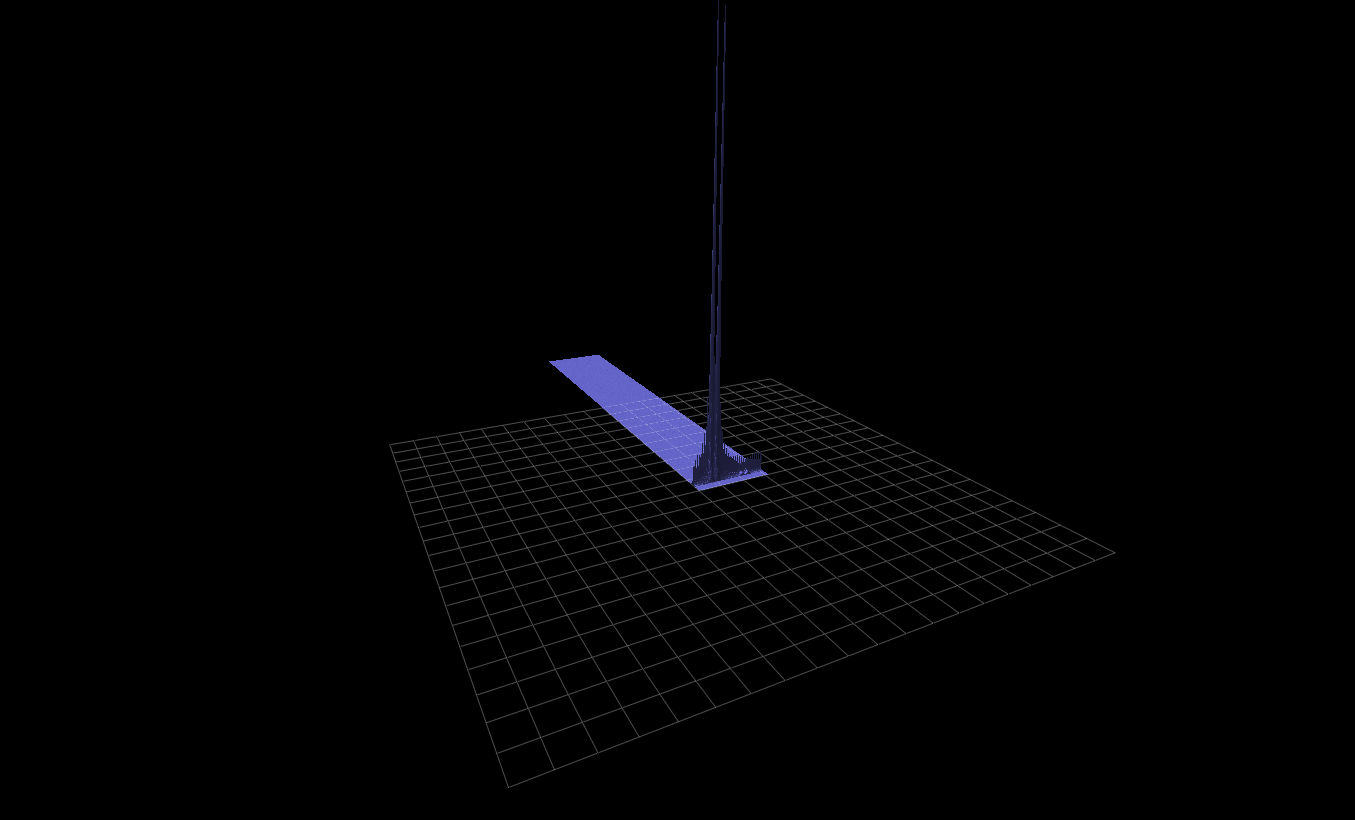
\includegraphics[width=\linewidth]{vector10-MTD-software.png}
		\caption{两目标速度差为10m/s}
		\label{fig:两目标速度差为10m/s}
	\end{subfigure}
	\quad
	\begin{subfigure}[H]{.45\linewidth}
		\centering
		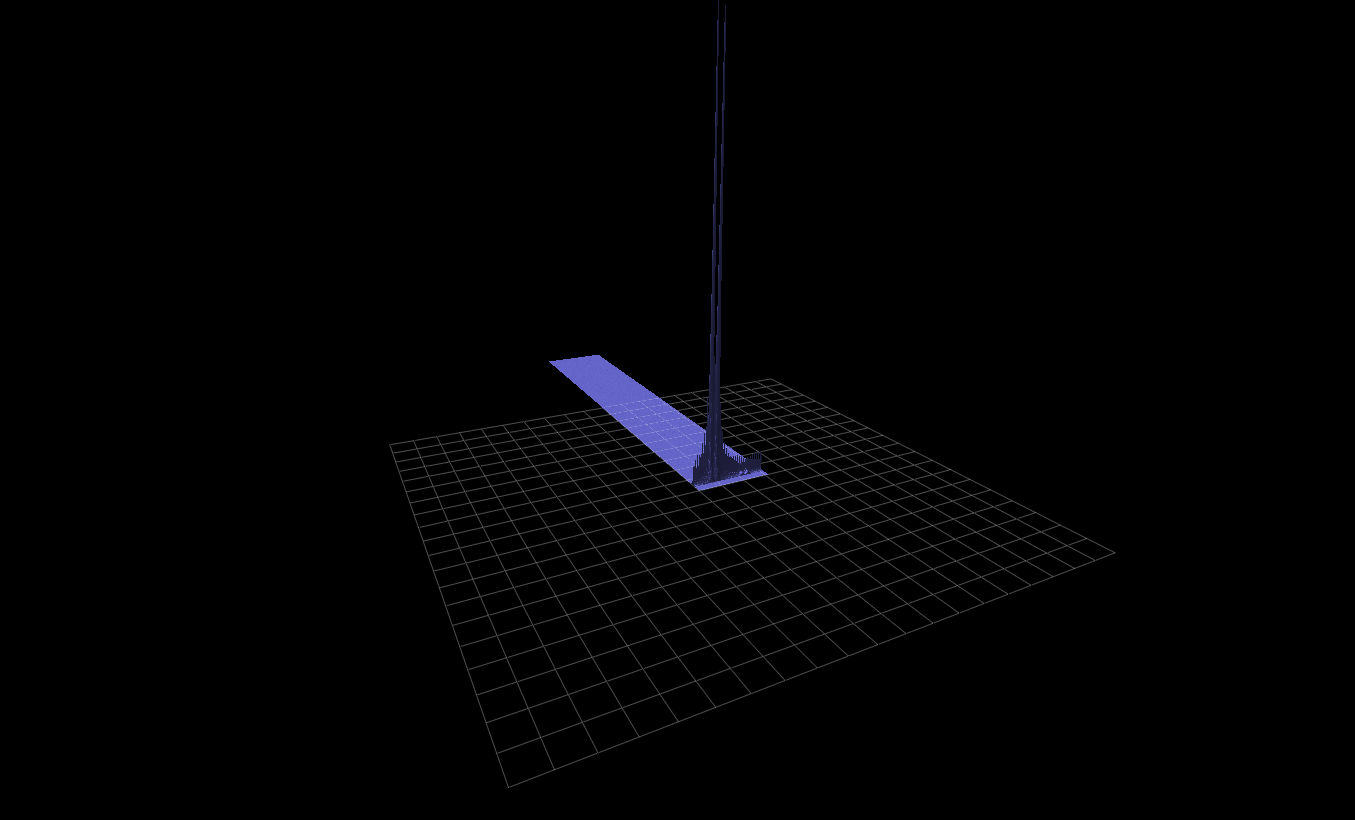
\includegraphics[width=\linewidth]{vector4-MTD-software.png}
		\caption{两目标速度差为4m/s}
		\label{fig:两目标速度差为4m/s}
	\end{subfigure}
	\quad
	\begin{subfigure}[H]{.45\linewidth}
		\centering
		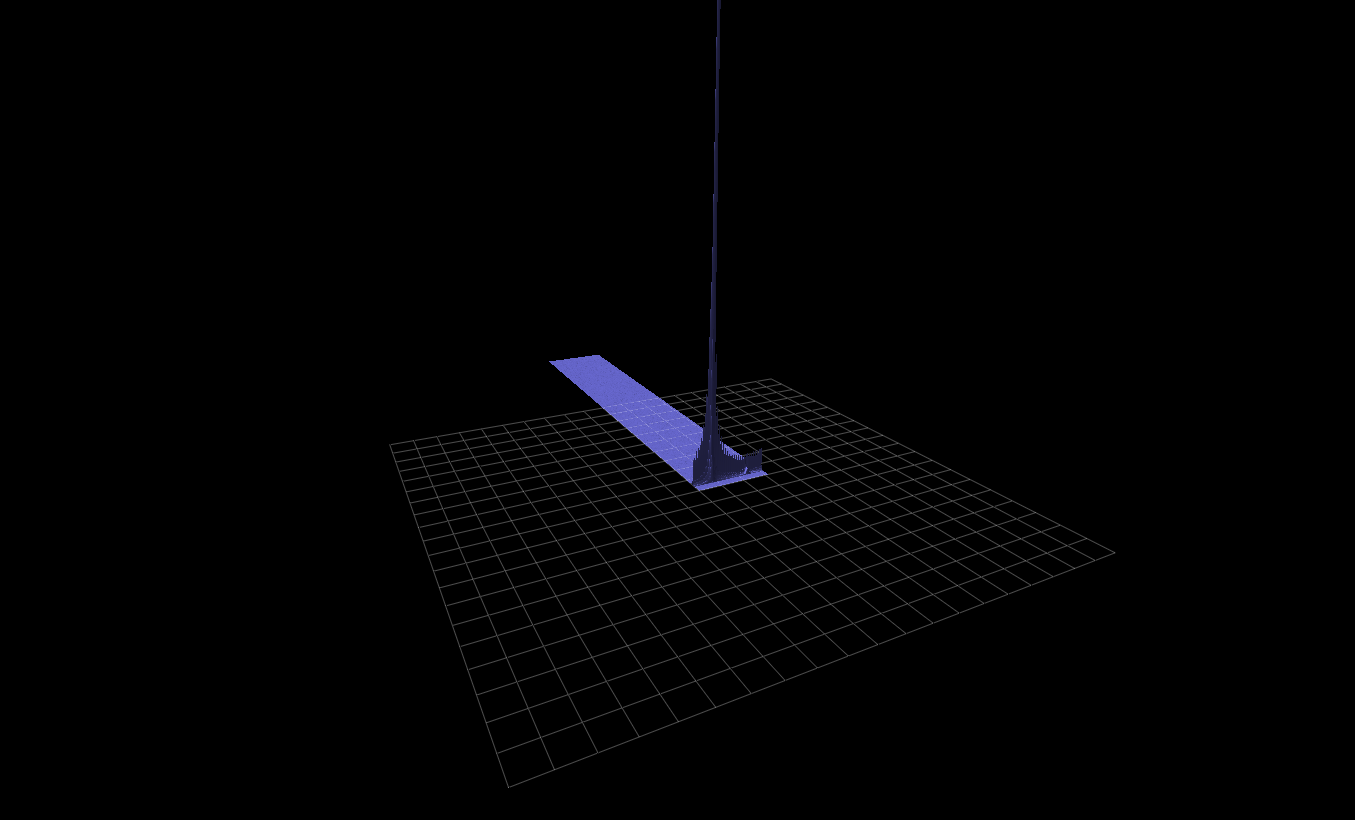
\includegraphics[width=\linewidth]{vector1-MTD-software.png}
		\caption{两目标速度差为1m/s}
		\label{fig:两目标速度差为1m/s}
	\end{subfigure}
	\caption{速度分辨}
	\label{fig:速度分辨}
\end{figure}

\subsection{距离分辨}%
\label{sub:距离分辨}

\begin{figure}[H]
	\centering
	\begin{subfigure}[H]{.45\linewidth}
		\centering
		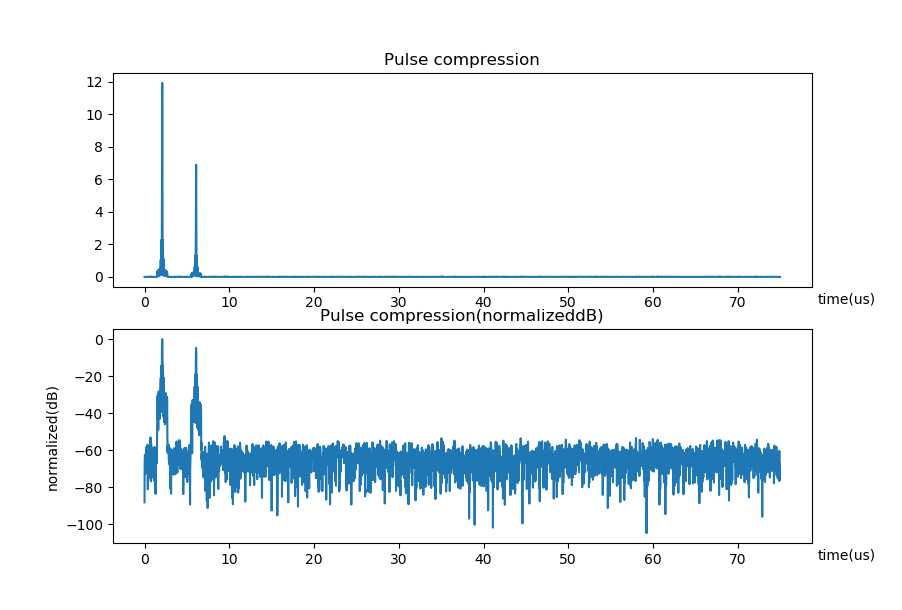
\includegraphics[width=\linewidth]{distance600-pulse-software.png}
		\caption{两目标距离差为600m}
		\label{fig:两目标距离差为600m}
	\end{subfigure}
	\quad
	\begin{subfigure}[H]{.45\linewidth}
		\centering
		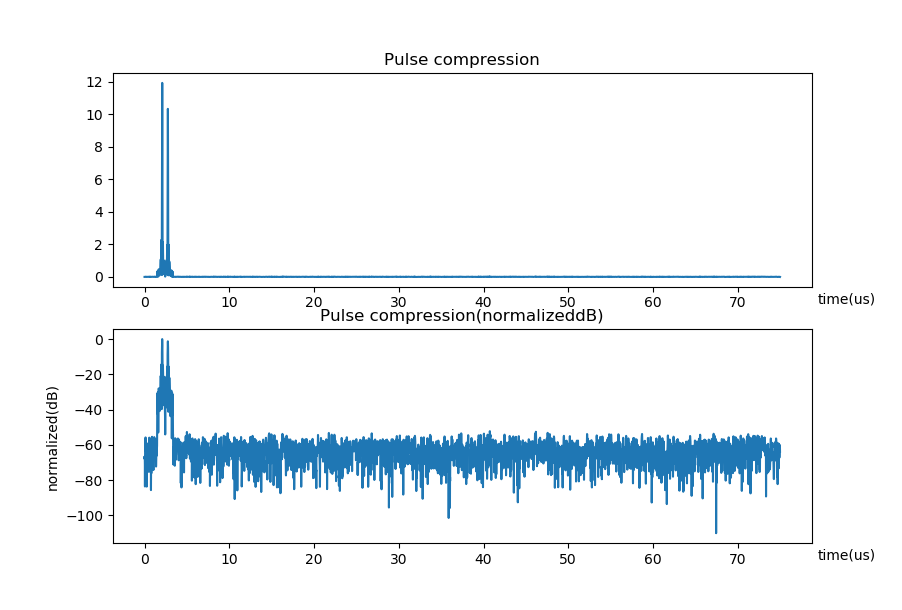
\includegraphics[width=\linewidth]{distance100-pulse-software.png}
		\caption{两目标距离差为100m}
		\label{fig:两目标距离差为100m}
	\end{subfigure}
	\quad
	\begin{subfigure}[H]{.45\linewidth}
		\centering
		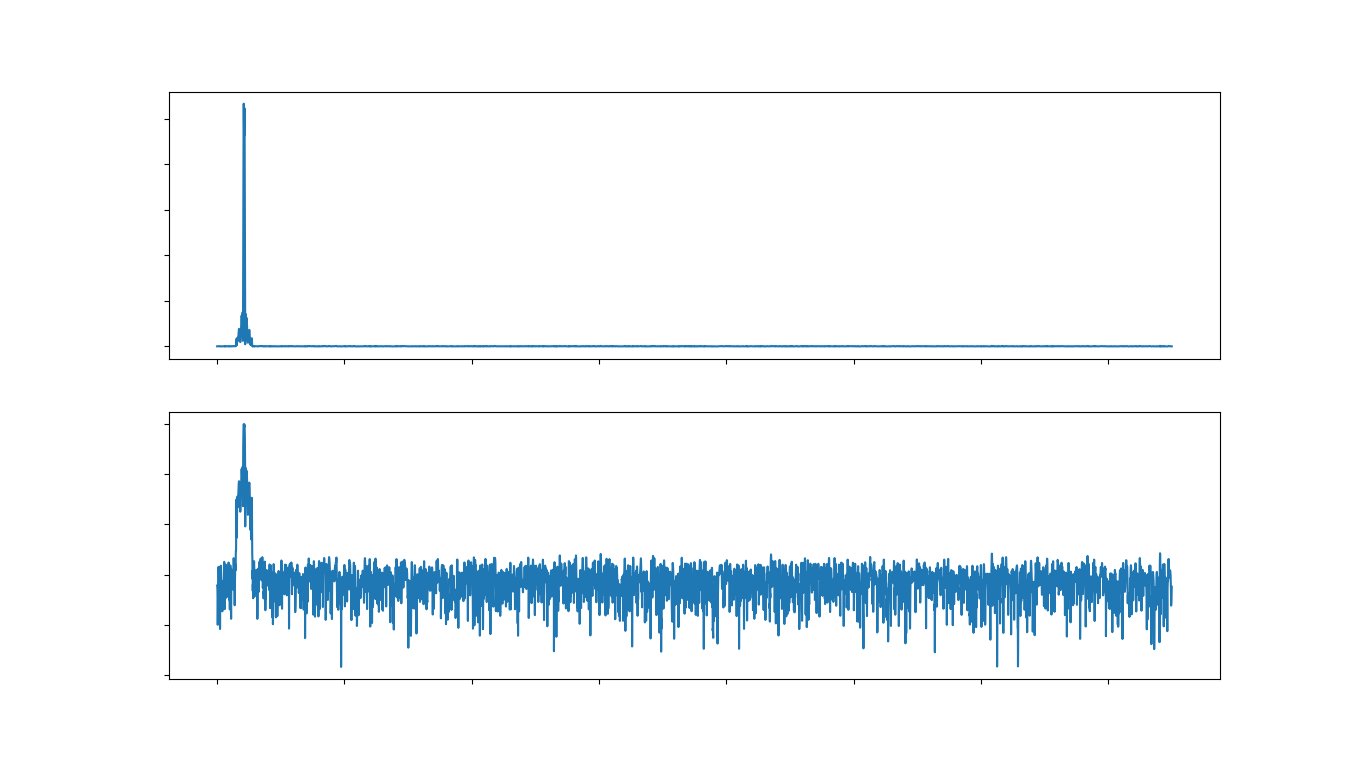
\includegraphics[width=\linewidth]{distance10-pulse-software.png}
		\caption{两目标距离差为10m}
		\label{fig:两目标距离差为10m}
	\end{subfigure}
	\quad
	\begin{subfigure}[H]{.45\linewidth}
		\centering
		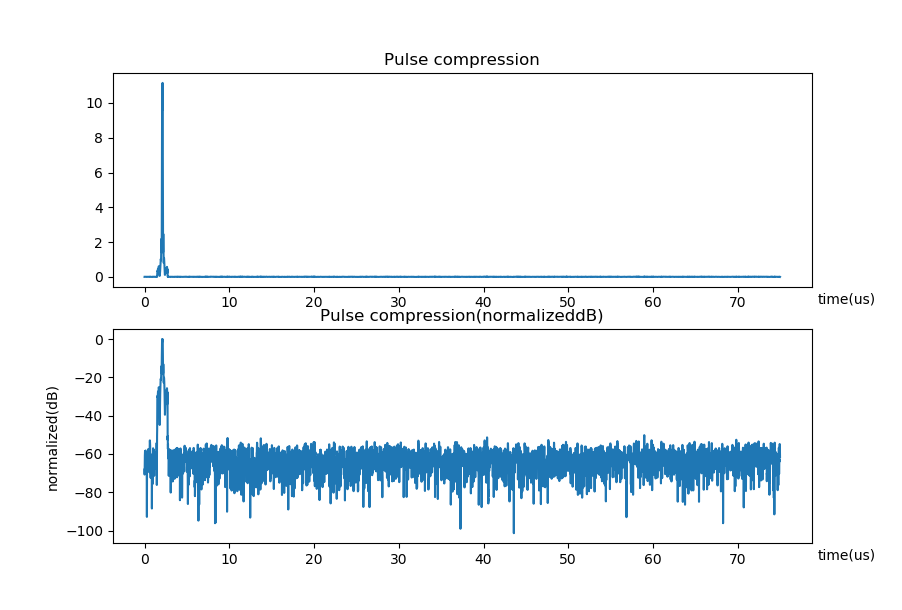
\includegraphics[width=\linewidth]{distance5-pulse-software.png}
		\caption{两目标距离差为5m}
		\label{fig:两目标距离差为5m}
	\end{subfigure}
	\caption{距离分辨}
	\label{fig:距离分辨}
\end{figure}

\section{实验感悟}%
\label{sec:实验感悟}

本次实验中遇到了以下问题:

\begin{enumerate}
	\item 对硬件设备的不了解。本实验使用的实验箱通过LAN线与上位机进行通讯。LAN线使用的RJ45接口有左右2边各有一个小灯,黄灯闪烁为上位机向实验箱传递数据,绿灯闪烁为上位机从实验箱下载数据。在实验之初因为不知道这个信息,导致上位机与实验箱连接出现问题时找不到原因,无从下手。
	\item 实验经验的匮乏。在采集示波器数据时没有记录哪张图片对应哪个参数,导致实验当时观察到了验证仿真的波形,但事后写实验报告时却找不到是哪一张图片。
\end{enumerate}

\newpage

% Fakesection 参考文献

\addcontentsline{toc}{section}{参考文献}

\bibliographystyle{IEEEtran}
\bibliography{bib/main}

% Fakesection 附录

\appendix

\section{代码}%
\label{sec:代码}

\subsection{单目标仿真}%
\label{sub:单目标仿真}

\langCVfile[Matlab][lst:one.m][Matlab]{one.m}{lst/one.m}

\subsection{双目标仿真}%
\label{sub:双目标仿真}

\langCVfile[Matlab][lst:two.m][Matlab]{two.m}{lst/two.m}

\subsection{单目标动态目标检测}%
\label{sub:单目标动态目标检测}

\langCVfile[Matlab][lst:oneMTD.m][Matlab]{oneMTD.m}{lst/oneMTD.m}

\subsection{双目标动态目标检测}%
\label{sub:双目标动态目标检测}

\langCVfile[Matlab][lst:twoMTD.m][Matlab]{twoMTD.m}{lst/twoMTD.m}

\end{document}

